\section{Introdução}
\label{sec:introduction}

O conceito da web semântica é uma ideia de Tim Berners-Lee: ``Web semântica é uma extensão da web comum em que a informação tem um melhor definido significado para os computadores e a cooperação das pessoas''~\cite{BernersLee01}. Em outras palavras, mudar a interconexão da web comum a um gigantesco banco de dados relacionado como é mostrado na Figura~\ref{fig:semantic_web} passando de uma abordagem orientada a arquivos (izquerda) a uma abordagem orientada a informação (direita).

\begin{figure}[H]
	\centering
	\begin{subfigure}{.45\textwidth}
		\centering
		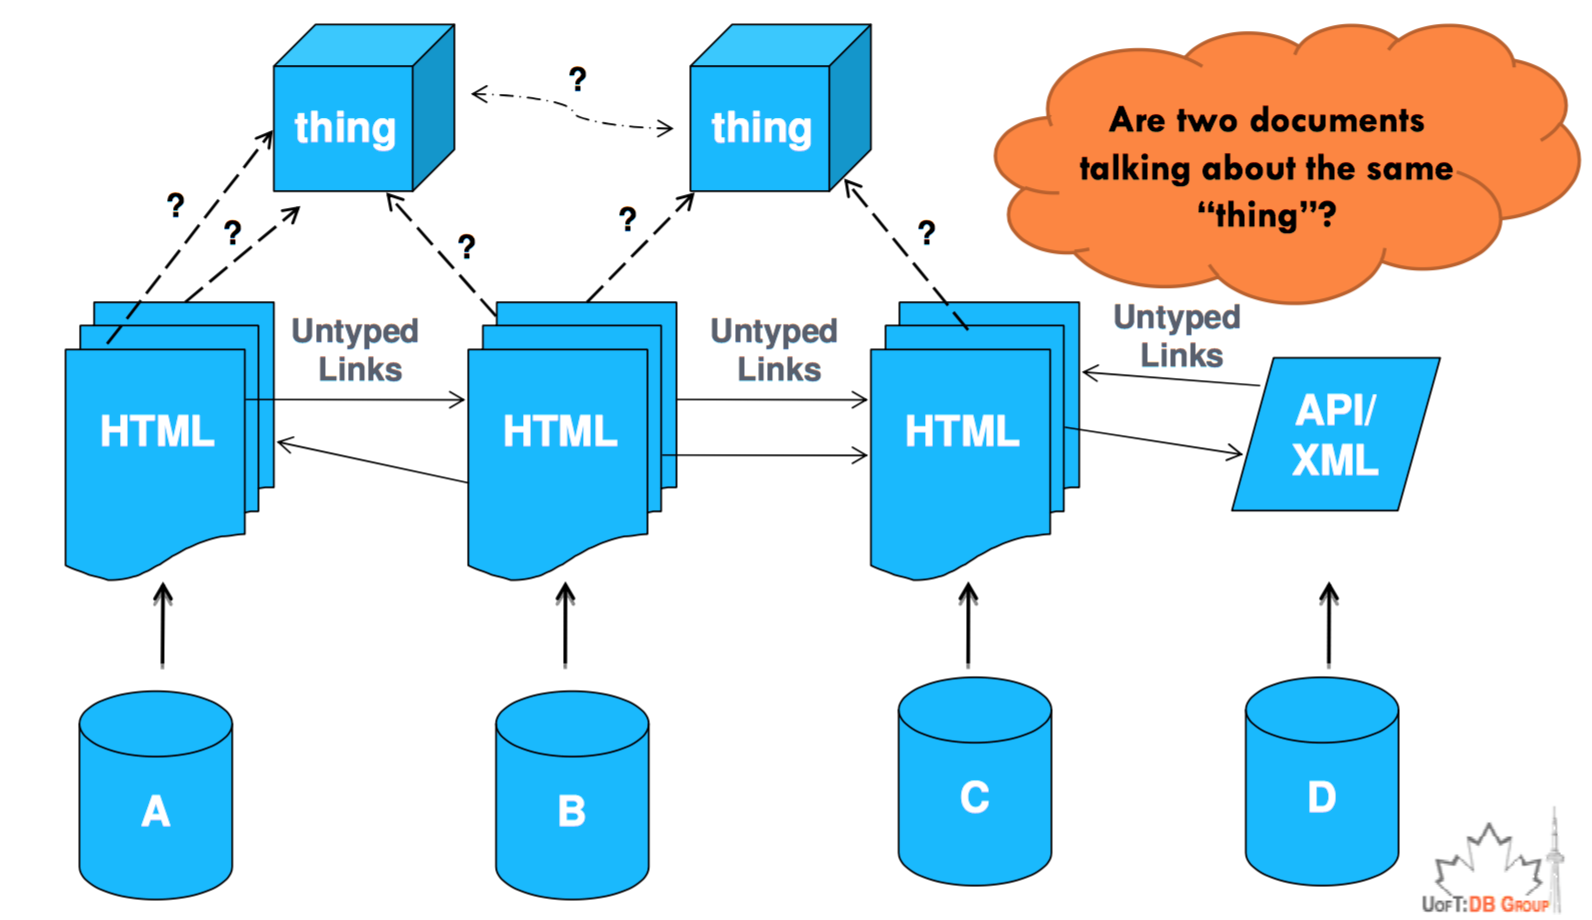
\includegraphics[height=3cm]{images/documentweb}
		%\caption{}
	\end{subfigure}
	\begin{subfigure}{.45\textwidth}
		\centering
		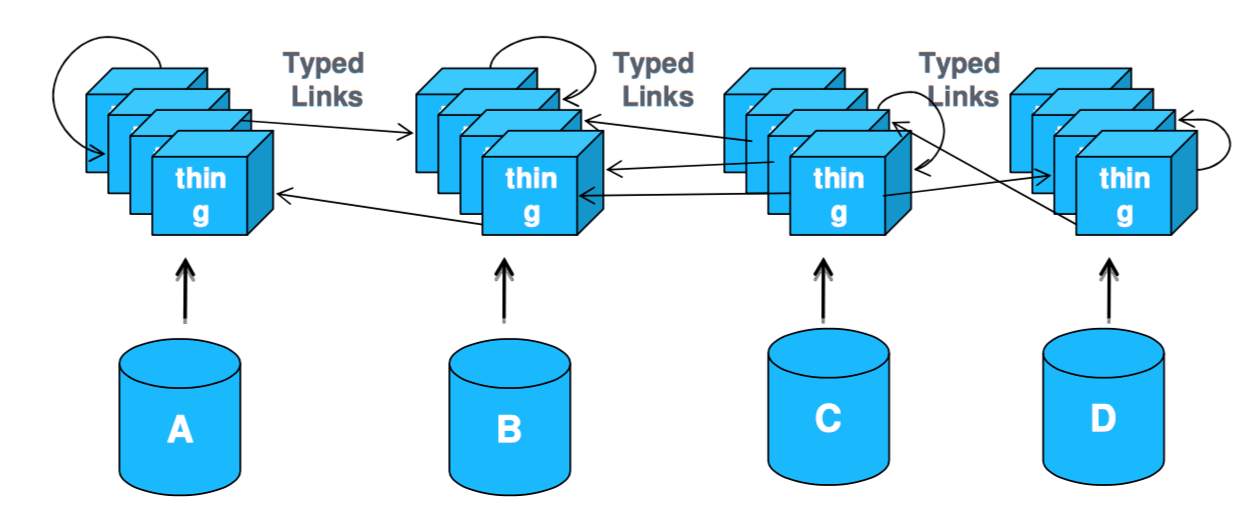
\includegraphics[height=3cm]{images/dataweb}
		%\caption{}
	\end{subfigure}
	\caption{Ideia da web semântica}
	\label{fig:semantic_web}
\end{figure}

O problema com aquela ideia de web semântica é que na web atual existem as seguintes situações:
\begin{itemize}
	\item Amplidão: Existem milhões de páginas
	\item Não definição única de termos: Existem termos como alto e jovem que são subjetivos
	\item Incerteza: Conceitos que tem incerteza, por exemplo sintomas de uma doença podem ser de alguma outra com outra probabilidade
	\item Inconsistência: Existem contradições lógicas
	\item Engano: A informação obtida não é sempre confiável
\end{itemize}

Ao longo deste trabalho, serão explicada a principal representação usada para a web semântica: ontologias, seus limitações e como aquele conceito foi extendido a ontologias probabilísticas para lidar com os desafios mencionados anteriormente. Finalmente, serão explicados alguns estudos feitos com aquele último conceito.